\subsection{Opsamling af accelerometer-signaler}\label{sec:acc_imp}

I dette projekt implementeres der på baggrund af krav opstillet i \autoref{sec:acc_teori} to analoge accelerometre ADXL335 fra Analog Devices. Accelerometerne er en triaksialt sensor, som har et arbejdsområde på minimum $\pm3~g$. Det analoge outputsignal er proportionalt med accelerationen \citep{analogdevices2009}. 

Det fremgår af databladet for accelerometrene at de skal forsynes med en spænding mellem $1,8~-~3,6~V$. Outputtet fra accelerometrene har et offset svarende til det halve forsyningsspændingen. Da accelerometerne forsynes med $3,3~V$ fra mikrokontrolleren, forventes offsettet at være på $1,65~V$,. Båndbredden og støjen varierer for akserne. For y-aksen ligger båndbredden mellem $0,5 - 1.600~Hz$ \fxnote{Den spektrale effekttæthed måles i $\mu g/$. Hvis dette divideres med kvadratroden af båndbredden af signalet $\sqrt{Hz}$, fås RMS af accelerationsstøjen ved en temperatur på $25^\circ$C} \citep{analogdevices2010}.

Accelerometrenes outputsensitivitet varierer ligefrem proportionelt med forsyningsspændingen. Sensitiviteten har et range der kan variere op til $10~\%$ \citep{analogdevices2010}. Ved en forsyningsspænding på $3,3~V$ er sensitiviteten $330~mV/g~\pm 10~\%$. 

\begin{figure}[H]
\centering
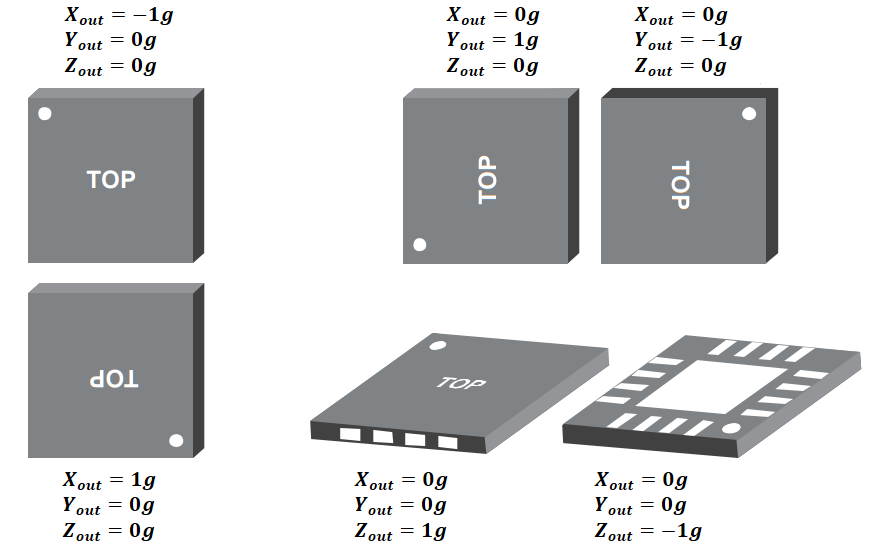
\includegraphics[width=0.85\textwidth]{figures/acc_paavirkning}
\caption{Påvirkning af accelerometeret i forskellige positioner. Til venstre måles accelerometeret lodret, til højre øverst måles det vandret og til højre nederst måles der i plan \citep{analogdevices2010}.}
\label{fig:acc}
\end{figure}

\noindent
Ved hældning af accelerometeret sker der en acceleration i forhold til tyngdekraften. Accelerations påvirkning der måles er afhængigt af retning og hældning af accelerometeret, hvilket fremgår af \autoref{fig:acc}. Hvis accelerometeret eksempelvis befinder sig i positionen, som er illustreret på \autoref{fig:acc} øverst til højre, påvirkes y-aksen med $\pm 1~g$ \citep{clifford2005}. Denne sammenhæng og derved patientens hældning kan udtrykkes ved \autoref{equ:vinkler}, hvor $\phi$ er vinklen i forhold til udgangspunktet for den pågældende akse \citep{clifford2005}.
\begin{equation} \label{equ:vinkler}
	V_{out} = V_{offset} + sensitivitet \cdot \sin(\phi)
\end{equation}